% !TeX root = exercise-2.tex
\documentclass[
  coursecode={CISC/CMPE 251},
  assignmentname={Exercise 2},
  studentnumber=20053722,
  name={Bryan Hoang}
]{
  ltxanswer%
}

\marksnotpoints{}

\usepackage{bch-style}

\begin{document}
  \begin{questions}
    \question[2]{}
    Use the Naive Bayes classifier as a predictor. Report results such as classification accuracy, confusion matrix, and perhaps some of the other measures we discussed.

    Explore the options for binning (that is converting a numerical attribute into a categorical one - really an ordinal one - by putting the values into ranges and calling each range a bin).

    Try this with at least one attribute in KNIME, with several different choices of bins, and see what effect this has on prediction performance.
    \begin{solution}
      For the exercise, I used the KNIME workflow, seen in Figure~\ref{fig:wine-workflow}, to predict the wine's type using all the attributes, and then assessed the use of binning to improve prediction results using on Flavanoids.

      Using the Naive Bayes classifier as a predictor with a 66\%/33\% partitioning for training and test data led to the model achieving a prediction accuracy of \textapprox{}96\%. As can be observed in Figure~\ref{fig:wine-confusion-matrix-base}, the confusion matrix shows that the model misclassified relatively few records.

      \begin{answerfigure}
        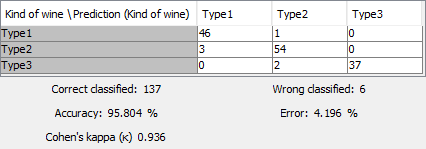
\includegraphics[width=0.75\textwidth]{wine-confusion-matrix-base.png}
        \captionof{figure}{Confusion matrix of the Naive Bayes predictor using all attributes}\label{fig:wine-confusion-matrix-base}
      \end{answerfigure}

      After filtering the data to only include the target attribute (wine type) and the Flavanoids, the model achieved a \textapprox{}77\% prediction accuracy, as shown in Fiture~\ref{fig:wine-confusion-matrix-flavanoids}.

      \begin{answerfigure}
        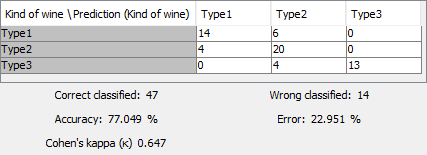
\includegraphics[width=0.75\textwidth]{wine-confusion-matrix-flavanoids.png}
        \captionof{figure}{Confusion matrix of the Naive Bayes predictor using only Flavanoids}\label{fig:wine-confusion-matrix-flavanoids}
      \end{answerfigure}

      \newpage

      I first tried manually binning the data after viewing the sorted the csv data along the Flavanoids column using the following intervals: \([0, 1.5], [1.5, 2.3], [2.3, \infty]\). I determined the endpoints  by looking for notable transitions in the wine type in the sorted data. The confusion matrix in Figure~\ref{fig:wine-confusion-matrix-binning-manual} shows that this method of binning increased the prediction accuracy by \textapprox{}3\%.

      \begin{answerfigure}
        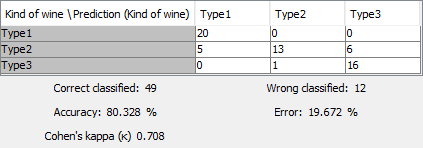
\includegraphics[width=0.75\textwidth]{wine-confusion-matrix-binning-manual.png}
        \captionof{figure}{Confusion matrix of the Naive Bayes predictor using 3 manually specified bins of Flavanoids data}\label{fig:wine-confusion-matrix-binning-manual}
      \end{answerfigure}

      Figure~\ref{fig:wine-confusion-matrix-binning-eq-freq} shows the confusion matrix using fixed frequency binning, which coincidentally gives the same prediction accuracy as the manually binned data, albeit with a slight difference in the misclassification between Type1 being Type2 and Type2 being Type3.

      \begin{answerfigure}
        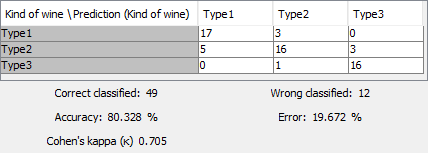
\includegraphics[width=0.75\textwidth]{wine-confusion-matrix-binning-eq-freq.png}
        \captionof{figure}{Confusion matrix of the Naive Bayes predictor using 3 fixed frequency bins of Flavanoids data}\label{fig:wine-confusion-matrix-binning-eq-freq}
      \end{answerfigure}

      The confusion matrix displayed in Figure~\ref{fig:wine-confusion-matrix-binning-eq-width} shows that the fixed width binning method gave a prediction accuracy of \textapprox{}60\%, which is the worst performing binning method by a relatively large margin.

      \newpage

      \begin{answerfigure}
        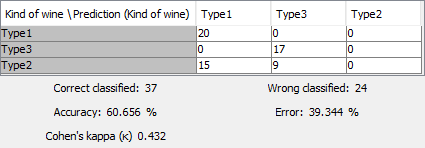
\includegraphics[width=0.75\textwidth]{wine-confusion-matrix-binning-eq-width.png}
        \captionof{figure}{Confusion matrix of the Naive Bayes predictor using 3 fixed width bins of Flavanoids data}\label{fig:wine-confusion-matrix-binning-eq-width}
      \end{answerfigure}

      \newpage

      \begin{answerfigure}
        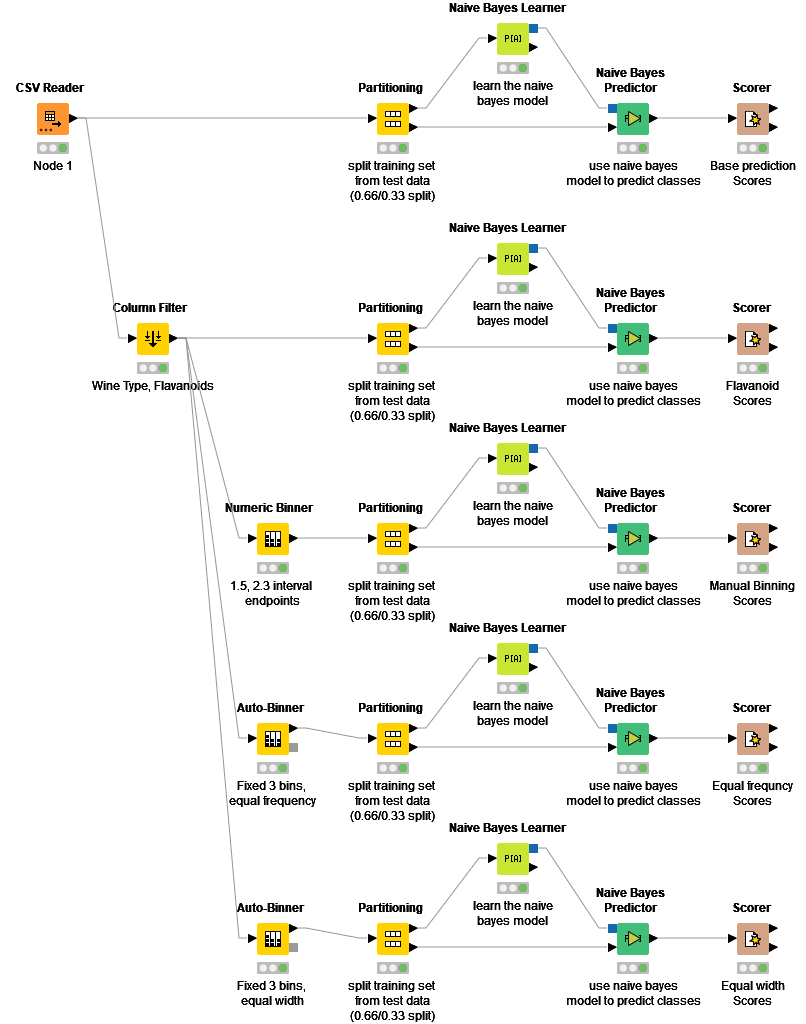
\includegraphics[width=\textwidth]{wine-bayes-predictor-workflow.png}
        \captionof{figure}{KNIME workflow used for analysis}\label{fig:wine-workflow}
      \end{answerfigure}
    \end{solution}
  \end{questions}
\end{document}
